\documentclass{standalone}
\usepackage{graphicx}	
\usepackage{amssymb, amsmath}
\usepackage{color}

\usepackage{tikz}
\usetikzlibrary{intersections, backgrounds, math}
\usepackage{pgfmath}

\definecolor{light}{RGB}{220, 188, 188}
\definecolor{mid}{RGB}{185, 124, 124}
\definecolor{dark}{RGB}{143, 39, 39}
\definecolor{highlight}{RGB}{180, 31, 180}
\definecolor{light_teal}{RGB}{107, 142, 142}
\definecolor{mid_teal}{RGB}{72, 117, 117}
\definecolor{dark_teal}{RGB}{29, 79, 79}
\definecolor{gray10}{gray}{0.1}
\definecolor{gray20}{gray}{0.2}
\definecolor{gray30}{gray}{0.3}
\definecolor{gray40}{gray}{0.4}
\definecolor{gray60}{gray}{0.6}
\definecolor{gray70}{gray}{0.7}
\definecolor{gray80}{gray}{0.8}
\definecolor{gray90}{gray}{0.9}
\definecolor{gray95}{gray}{0.95}

\begin{document}

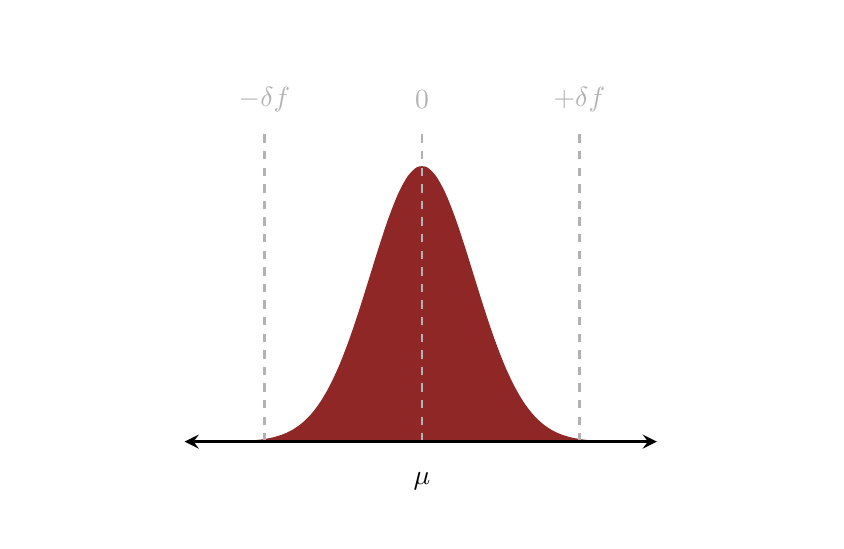
\begin{tikzpicture}[scale=1.0]

  \begin{scope}[shift={(0, 0)}]
    \draw[white] (-5, -3) rectangle (5, 3.25);

    \fill[domain={-3:3}, smooth, samples=50, line width=1, variable=\x, color=dark] 
          plot ({\x},{3.5 * exp(- (\x / 0.927) * (\x / 0.927)) - 2});

    \draw[gray70, dashed, line width=1] (+ 2, -2) -- (+ 2, 2);
    \draw[gray70, dashed, line width=1] (0, -2) -- (0, 2);
    \draw[gray70, dashed, line width=1] (- 2, -2) -- (- 2, 2);
    \node[gray70] at (0, 2.35) { $0$ };
    \node[gray70] at (0 - 2, 2.35) { $-\delta f$ };
    \node[gray70] at (0 + 2, 2.35) { $+\delta f$ };

    \draw [<->, >=stealth, line width=1.25] (-3.015, -2.00) -- +(6, 0);
    \node at (0, -2.5) { $\mu$ };
  \end{scope}
  
\end{tikzpicture}

\end{document}  